\skriptsection{Komplexe Zahlen}{1}
\skriptsubsection{Grundlagen}{1ff}
\begin{minipage}[t]{9.4cm}
	\textbf{Kartesische Form}\\
	Normalform: $z = z_1 +j z_2$\\
	$z_1 = \text{Re}(z), \quad z_2 = \text{Im}(z)$\\
	Umrechnung in Polar:\\
	$r = |z| = \sqrt{z_1^2 + z_2^2}, \quad 
	\varphi = 	\begin{cases} 
                	\arctan(\frac{z_2}{z_1}) &z_1 \geq 0\\
                	\pi + \arctan(\frac{z_2}{z_1}) &z_1 < 0
    			\end{cases}$
\end{minipage}
\begin{minipage}[t]{9.4cm}
	\textbf{Polarsystem}\\
	Polarform: 
	$z = r \cjs(\varphi) = r(\cos{\varphi} + j\sin{\varphi}) = r e^{j \varphi}$\\
	$\varphi = \arg(z)$

	Umrechnung in Kartesisch:\\
	$z_1 = |z| \cos{\varphi}, \quad z_2 = |z| \sin{\varphi}$
\end{minipage}

$\textbf{Imaginäre Einheit:} \qquad j^2 = -1 \qquad e^{j\pi} = e^{-j\pi} = -1 \qquad e^{j2\pi} = 1 \qquad \frac{1}{j} = -j \qquad e^{j\frac{\pi}{2}}= j \qquad j^j = e^{-\frac{\pi}{2}+2k\pi}$

\vspace{-\baselineskip}
\skriptsubsection{Rechenregeln}{10ff}
\renewcommand{\arraystretch}{1.5}
\begin{tabular}{| l | l |}
\hline
	$+, -$
	& Selbige Regeln wie für $\mathbb{R}$\\

\hline
	Multiplikation
	&$a \cdot b = 
		|a| |b| \cjs(\alpha + \beta) = 
		|a| |b| e^{j(\alpha + \beta)}$ (kartesisch: $a_1 \cdot b_1 = (a_1 \cdot b_1 - a_2 \cdot b_2) + j \cdot (a_1 \cdot b_2 + a_2 \cdot b_1)$)\\

\hline
	Division
	&$\frac{a}{b} = 
		\frac{\left|a\right|}{\left|b\right|} \cjs(\alpha - \beta) =
		\frac{\left|a\right|}{\left|b\right|} e^{j(\alpha - \beta)}$ (kartesisch: Mit
		konj. komplex des Nenners erweitern) \\

\hline
	Konjugiert komplex
	&$\overline{z} = \overline{z_1 + jz_2} = z_1 - jz_2; \qquad \qquad z \cdot \overline{z} = |z|^2$\\

\hline
	Wurzeln
	&$\sqrt[n]{a} = \sqrt[n]{|a|} \cjs(\frac{arg(a)}{n}+k\frac{2\pi}{n}) = 
	\sqrt[n]{|a|} e^{j(\frac{\alpha}{n} + k \frac{2\pi}{n})} \quad (k = 0, 1,
	\ldots, n-1 \Rightarrow \text{n Lösungen in } \mathbb{C} !)$ \\

\hline
	Potenzen
	&$a^n = |a|^n \cjs(n\alpha) = 
	|a|^n e^{jn\alpha}$\\

\hline
	$e^z$ &$e^{z_1+jz_2} = e^{z_1} \cjs(z_2) = e^{z_1} (\cos{z_2} + j\sin{z_2})$ ; $|e^z| = e^{z_1}$ ; $arg(e^z) = z_2$\\
	
\hline
	Moivre'sche Formel
	&$\text{cjs}^n(\varphi) =
	(\cos{\varphi} + j\sin{\varphi})^n = 
	\cos(n\varphi) +j\sin(n\varphi) \quad (n \in \mathbb{N})$\\

\hline
	Logarithmus
	&$Ln(z) = \ln{|z|} + j (\arg(z) + 2k \pi)=\ln|a|+j\arg(a) \qquad a^b = e^{b\cdot Ln(a)} \rightarrow$ (keine Potenzgesetze) \\

\hline
	& $\frac{1}{\cjs{\varphi}} = \cjs{-\varphi} \qquad cjs(\varphi)^n = cjs(n\varphi)$ \\
\hline
\end{tabular}
\renewcommand{\arraystretch}{1}\\

\begin{minipage}[t]{11.4cm}
	\textbf{Bemerkungen}
	\begin{itemize}
	  \item $p_n(z) \; (n \geq 1, z \in \mathbb{C})$ hat $n$ Lösungen und Nullstellen (in
	$\mathbb{C}$)  
	  \item Allgemeine Potenzen $a^b,\;a,b \in \mathbb{C}$ können mit $e^{b \cdot 
	  Ln(a)}$ und den bekannten für $\mathbb{R}$ gültigen Potenzregeln gelöst
	  werden.
	  \item Re$\left (\frac{a}{b} \right) = 0$: Die beiden kompl. Zahlen $a, b$
	  stehen senkrecht zueinander.
	\end{itemize}
\end{minipage}
\begin{minipage}[t]{7.4cm}
	\textbf{Einheitswurzeln}\\
	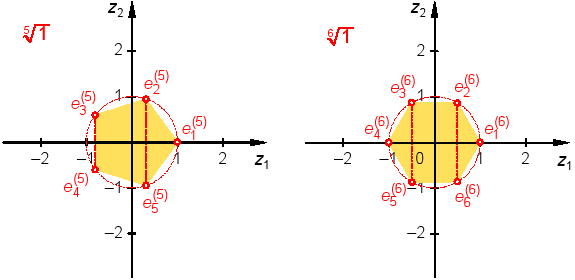
\includegraphics[width=7cm]{./bilder/einheitswurzel.png}
\end{minipage}

\vspace{-\baselineskip}
\subsection{12. Einheitswurzeln ($(k - 1) \cdot 30^{\circ}$)}
$e^{(12)}_1 = 1,\;
	e^{(12)}_2 = \frac{\sqrt3}{2} + \frac12j,\;
	e^{(12)}_3 = \frac12 + \frac{\sqrt3}{2}j,\;
	e^{(12)}_4 = j,\;
	e^{(12)}_5 = -\frac12 + \frac{\sqrt3}{2}j,\;
	e^{(12)}_6 = -\frac{\sqrt3}{2} + \frac12 j,\\
	e^{(12)}_7 = -1,\;
	e^{(12)}_8 = -\frac{\sqrt3}{2} - \frac12 j,\;
	e^{(12)}_9 = -\frac12 - \frac{\sqrt3}{2}j,\;
	e^{(12)}_{10} = -j,\;
	e^{(12)}_{11} = \frac12 - \frac{\sqrt3}{2}j,\;
	e^{(12)}_{12} = \frac{\sqrt3}{2} - \frac12j$

\subsection{Nullstellen von Polynomen}
Ein komplexes Polynom p(z) von Grad $n$ hat in $ \mathbb{C} $ genau $n$ Nullstellen.\\
Alle diese Nullstellen liegen in einer Kreisscheibe um den Ursprung mit dem Radius $r = \sum\limits_{k=0}^{n} \left| \frac{a_k}{a_n} \right| = \left| \frac{a_0}{a_n} \right| + \left| \frac{a_1}{a_n} \right| + ... + \left| \frac{a_n}{a_n} \right|$ \\ \\
Bei Polynomen mit reellen Koeffizienten treten nicht-reelle Nullstellen immer als konj.-kompl. Paare ($z_0$ und $\bar{z_0}$) auf.\\
Ein Polynom mit reellen Koeffizienten von \textit{ungeradem} Grad hat mind. eine \textit{reelle} Nullstelle.\\
Bei Polynomdivision immer mit reellen Zahlen arbeiten; konj.-kompl. Paare zusammenfassen.\\
\textbf{Berechnung:}\\
\begin{tabular}{l l}
	quadr. Polynome & Polynome mit $a_n = 1, a_{n-1} = a_{n-2} = ... = a_1 = 0, a_0 = a$\\
	$p(z) = az^2 + bz + c = 0$ & $p(z) = z^n + a = 0$\\
	$z_{1,2} = \frac{-b \pm \sqrt{b^2 -4ac}}{2a}$ & $z_k = \sqrt[n]{|a|} \cdot cjs(\frac{\varphi_a+\pi}{n} + (k-1) \cdot \frac{2\pi}{n})$ mit $k = 1, 2, ..., n$ 
\end{tabular}

\skriptsubsection{Euler}{30f}
\renewcommand{\arraystretch}{1.5}
\begin{tabular}{| l | l | l | l | l | l |}
\hline
	$\sin{\alpha} = \frac{e^{j\alpha} - e^{-j\alpha}}{2j}$ &

	$\cos{\alpha} = \frac{e^{j\alpha} + e^{-j\alpha}}{2}$ &

	$\tan{\alpha} = \frac{\sin \alpha}{\cos \alpha} = -j \frac{e^{j\alpha}-e^{-j\alpha}}{e^{j\alpha}+e^{-j\alpha}}$ & 

	$\sinh{\alpha} = \frac{e^\alpha - e^{-\alpha}}{2} $ &

	$\cosh{\alpha} = \frac{e^\alpha + e^{-\alpha}}{2} $ & 
	
	$\tanh{\alpha} = \frac{\sinh{\alpha}}{\cosh{\alpha}}$\\
\hline
\end{tabular}
\renewcommand{\arraystretch}{1}

\skriptsubsection{Überlagerung von harmonischen Schwingungen}{32f}
$$A \cdot \sin(\omega t + \varphi) = Im[A \cdot e^{j(\omega t + \varphi)}] =
Im[\underbrace{A \cdot e^{j\varphi}}_{\text{\tiny{Complexe Amplitude}}}
\cdot \underbrace{e^{j\omega t}}_{\text{\tiny{Zeitfunktion}}}]$$
%
%Alle komplexen Schwingungen in kartesische Form umwandeln und addieren, danach
%wieder zurück in Polarform $ A_{total} \cdot e^{j\varphi}$ zurückwandeln.
%
$$ A_1 \cdot \sin(\omega t + \varphi_1) + A_2 \cdot \cos(\omega t + \varphi_2) 
 \quad \Rightarrow \quad 
 Im[A_1 \cdot e^{j(\omega t + \varphi_1)} + A_2 \cdot e^{j (\omega t + \varphi_2
 + \frac{\pi}{2})}] \quad \Rightarrow \quad 
 Im[e^{j \omega t} \cdot  (A_1 \cdot e^{j \varphi_1} + A_2 \cdot e^{j (\varphi_2
 + \frac{\pi}{2})}]$$ 
Komplexe Amplituden in kartesische Form umwandeln, zusammenzählen und wieder
zurück in Polarform wandeln.
$$ Im[e^{j \omega t} \cdot  (A_{total} \cdot e^{j \varphi_{total}})] 
 \quad \Rightarrow \quad 
 Im[A_{total} \cdot e^{j (\omega t + \varphi_{total})}] 
 \quad \Rightarrow \quad 
 A_{total} \cdot \sin(\omega t + \varphi_{total})$$ 
$$A = |A_1 \cdot e^{j\varphi_1} + A_2 \cdot e^{j\varphi_2}| \qquad \varphi = arg(A_1 \cdot e^{j\varphi_1} + A_2 \cdot e^{j\varphi_2})$$
